\chapter{FHP}
The first upgrade of HPP bears name after its inventors -- Frisch, Humpfrey and Pomeu. 
They published it in 1986 together with its 3D brother FCHC, that we will analyze later, in this chapter we will stick to 2D model.


As any experienced gamer knows, 2D plane can be uniformly covered by hexagons.

If we chose hexagonal grid as the lattice for HPP-like automaton, we get the FHP.

On the Figure \ref{FHPgrid}, we see part of this hexagonal lattice. The dots represent the nodes.
On this figure, six lattice vectors points from one of the nodes into the neighbouring nodes.
\begin{figure}[htbp] \label{FHPgrid}
 \centering
 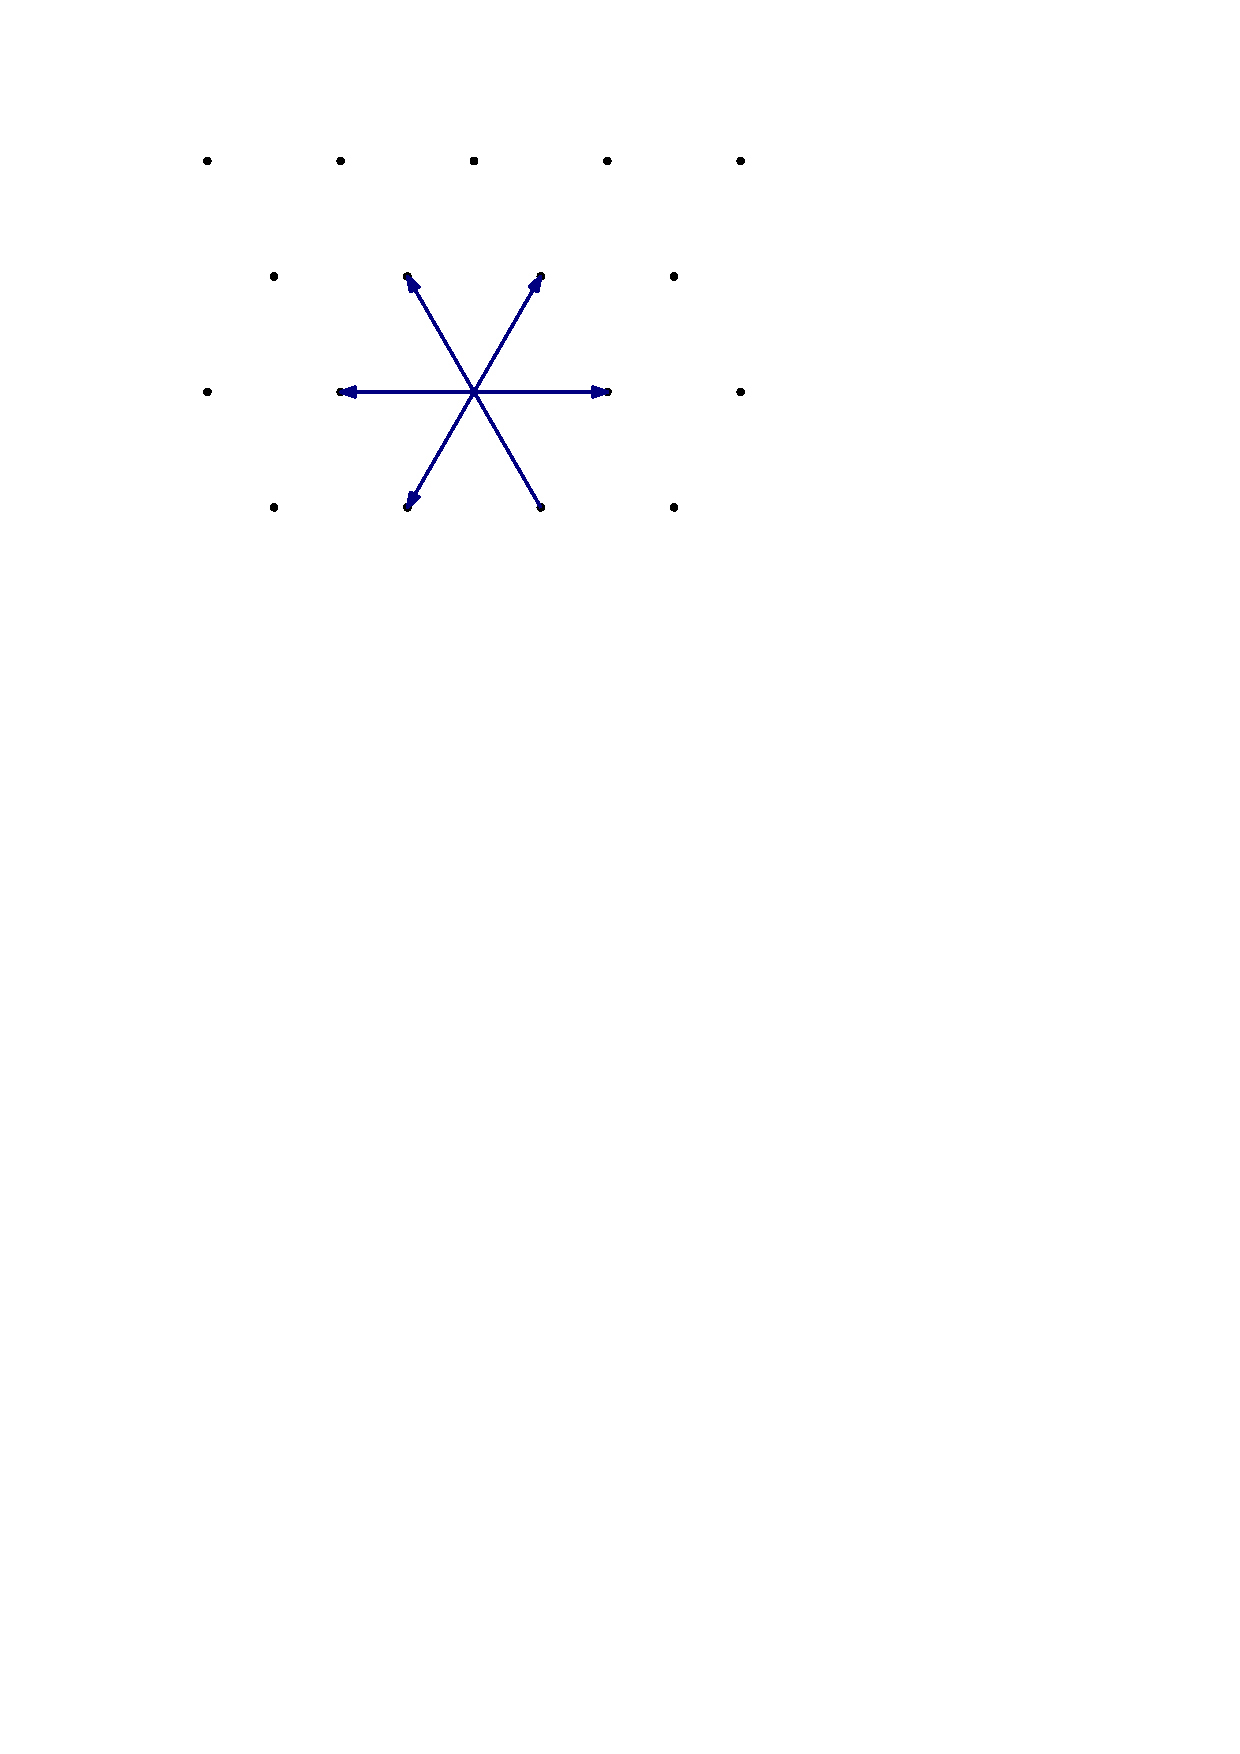
\includegraphics[width=0.4\textwidth]{./img/fhp-desc}
 
\end{figure}

Six lattice vectors per node imply that each node consists of six cells. Each of these cells can be occupied by one particle, that propagates along the lattice vectors to its neighbors.

\section{Update rule}
As in HPP (and any LGCA that we will study), update consists of two subsequent steps, collision and propagation.
Propagation phase is straigt-forward - if the cell is occupied by one particle
In the intersection of lines, we have nodes consisting of six cells.\\

So we have mesh with better (suffiecient!) rotational symmetry and nodes with richer and more interesting set of configurations.\

And among these configurations is one that does not conserve number of particles in opposite directions, see Figure~\ref{symm}.\

\begin{figure}[htbp]
 \centering
 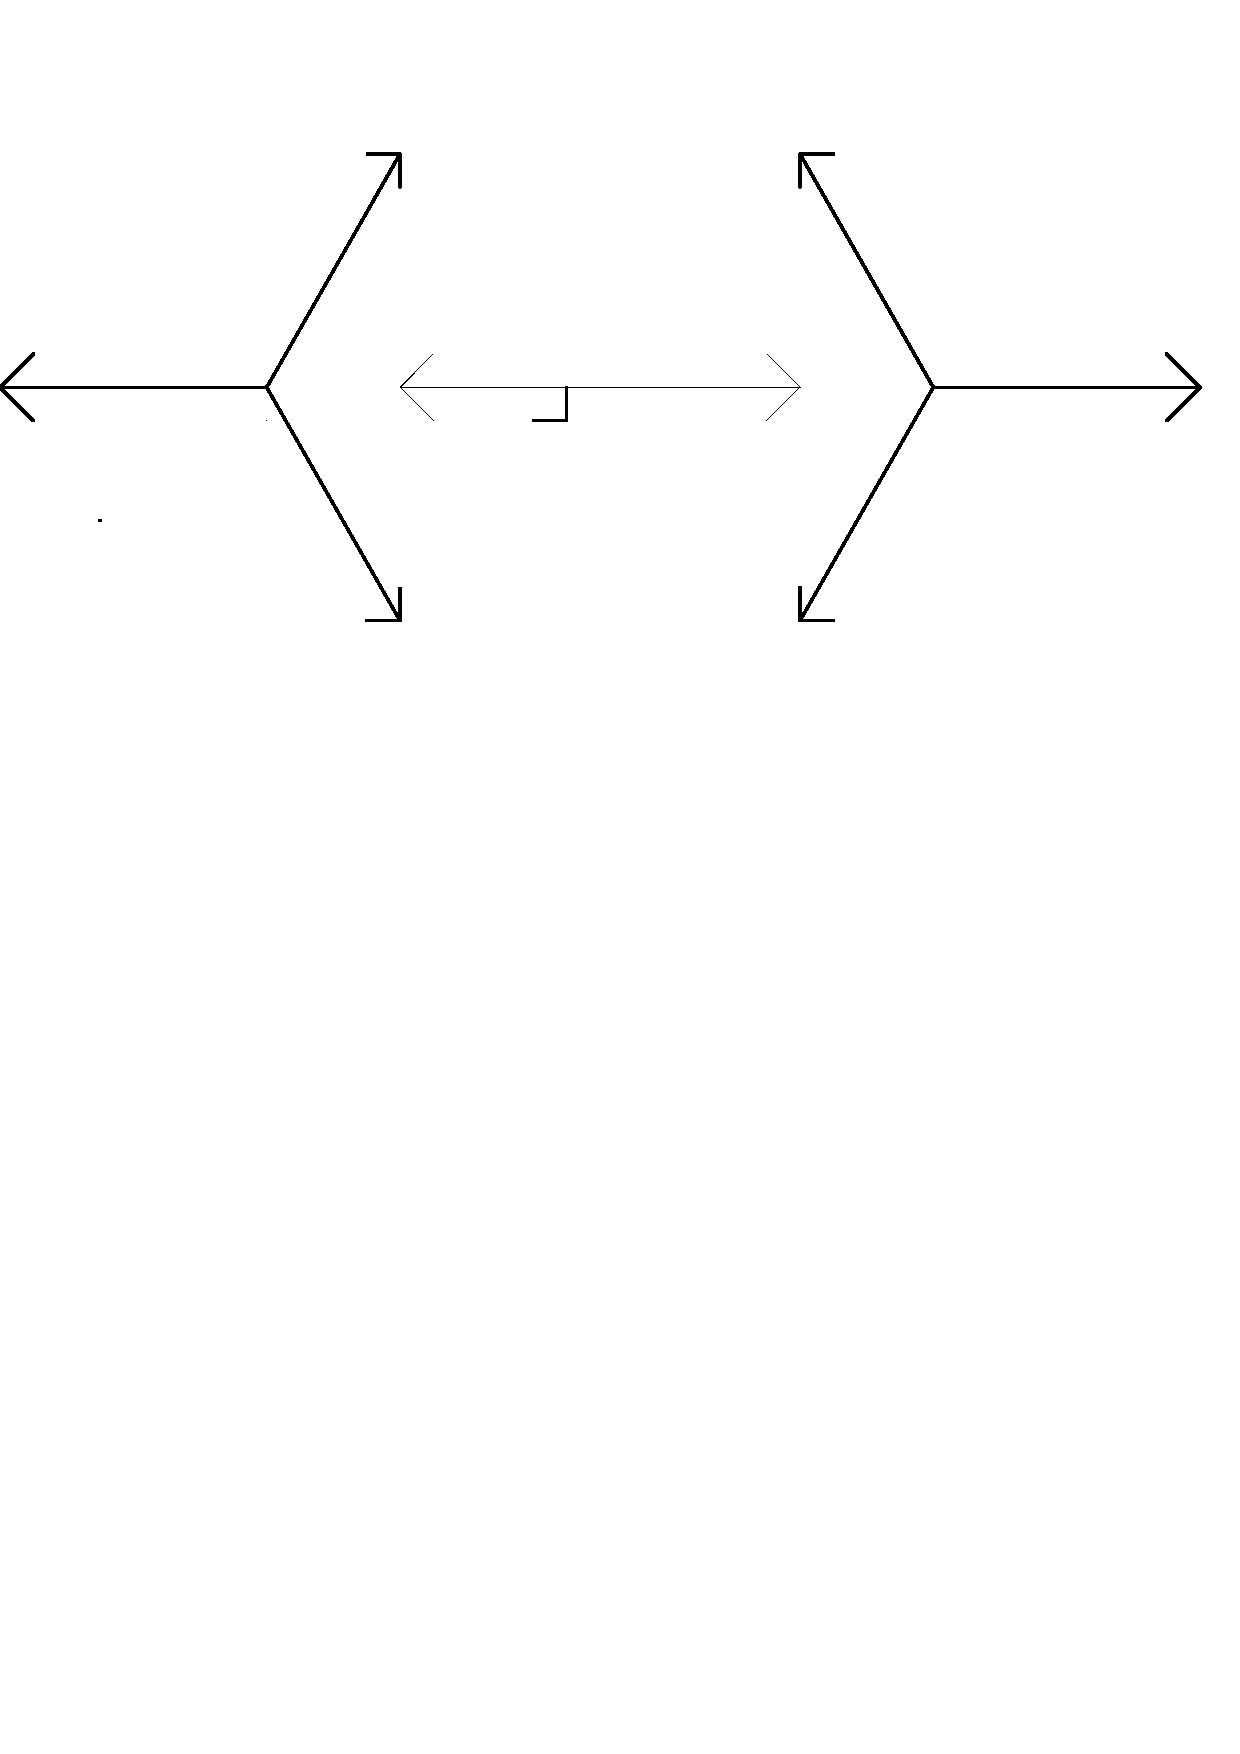
\includegraphics[width=0.4\textwidth]{./img/fhp_sym_col}
 \caption{Symetric colision of 3 particles}
 \label{symm}
 
\end{figure}


%Do we have collision configurations that do not conserve these quantity in fhp?
%is there a way to resolve this problems?

This is the only symetric colison, however.
For other colisions - see figures below, we have two states that are offering.
If we are chosing randomly from these,
we get rid of other spurious invariants.
(maybe we should choose more careful statements, as there exists spurious invariants for any type of FHP, 
but these invariants are under level of the noise, 
and they are not hapenning in collisions with obstacles, 
and regions around obstacles interest us most).\\

%In hpp, there exist only one colision configuration, and it has a bad property: it does not change number of particles in oposite dirrections.
%fortunately, there is one (picture)

At least in the rough way, we showed how FHP works.
In the next chapter, we are going to PROVE FHP really works - prove that FHP converges to Navier-Stokes equations.